Dans cette section, nous allons d'abord présenter ce qu'on appelle les ``eigenfaces''.
Nous allons ensuite faire une brève présentation de la méthode de classification
``bayésien naïf''. Nous exposerons alors les différentes étapes de la méthode proposée
par \cite{article} ainsi que les résultats obtenus. Nous finirons par une critique de
la démarche de test de \cite{article}.


\subsection{Présentation des eigenfaces} \label{subsection:presentation_eigenfaces}
Soit un ensemble d'images de visages. On transforme chaque image, qui est un signal
discret à deux dimensions, en un vecteur à une dimension (on travaille avec des
images en niveaux de gris). On calcule alors la matrice de variance-covariance
de ces vecteurs. On appelle eigenfaces les vecteurs propres de cette matrice.

Plus formellement : soit l'ensemble d'images $\{I_1, I_2, ..., I_M\}$.
Les étapes pour trouver les eigenfaces sont :
\begin{enumerate}
    \item Transformer chaque image $I_i$, qui est en deux dimensions,
    en un vecteur $\Gamma_i$ à une dimension.
    \item Calculer le vecteur moyen $Y$ : $Y = \frac{1}{M} \sum_{i=1}^M \Gamma_i$.
    \item Soustraire le vecteur moyen $Y$ de chaque vecteur $\Gamma_i$ : $\phi_i = \Gamma_i - Y$.
    \item Calculer $C$, la matrice variance-covariance des vecteurs $(\phi_i)_{i=1}^M$ :
    $C = A^TA$, où la ligne $i$ de $A$ est $\phi_i$.
    \item Calculer la matrice $u$, dont chaque colonne correspond à un vecteur
    propre de $C$. Les colonnes de $u$ sont les eigenfaces.
\end{enumerate}
Si $N$ est le nombre de pixels d'une image, alors $C$ est une matrice $N \times N$.
Pour $N$ assez grand (ce qui est très souvent le cas quand on travaille sur des images),
le calcul des vecteurs propres de $C$ devient vite très coûteux. Au lieu de faire cela,
on calcule les vecteurs propres de $AA^T$ (ils sont au nombre de $M$, le nombre d'images,
sachant que dans la plupart des cas $M << N$). Alors, pour chaque vecteur propre $v$ de
$AA^T$, $u = Av$ est un vecteur propre de $C$. Ça nous permet d'obtenir $M$ vecteurs
propres ($M$ étant le nombre d'images) qui sont considérés les eigenfaces et qui forment
une base de l'espace vectoriel des images.


\subsection{Classification bayésienne}
Soit un problème de classification où les individus sont représentés
par la variable aléatoire $X$ et les classes par la variable aléatoire $Y$.
La classification bayésienne repose sur le fait de classer un individu $x$ dans la
classe $y$ qui maximise la probabilité : $P(Y=y|X=x)$.

Le théorème de Bayes nous dit que :
\[
    P(Y=y|X=x) = \frac{P(X=x|Y=y) \times P(Y=y)}{P(X=x)}
\]
Donc pour maximiser $P(Y=y|X=x)$, il suffit de maximiser $P(X=x|Y=y) \times P(Y=y)$
(puisque $P(X=x)$ ne dépend pas de $y$ et nous cherchons à maximiser selon $y$).
On peut facilement estimer $P(Y=y)$ (par un simple comptage dans l'échantillon par exemple).
Le problème réside dans le calcul de $P(X=x|Y=y)$ sachant que $X$ est dans $\mathbb{R}^d$, 
c.a.d. que $X = (X_1, X_2, ..., X_d)$ où $X_i \in \mathbb{R}$.

L'hypothèse ``naïve'' sur laquelle se base la classification bayésienne est de supposer
les variables aléatoires $X_i$ indépendantes (d'où le nom ``bayésien naïf'' ou ``naive bayes''
en anglais). Quand on fait cette hypothèse, il devient plus facile de calculer $P(X=x|Y=y)$.
En effet :
\[
    P(X=x|Y=y) = P(X_1=x_1, X_2=x_2, ..., X_d=x_d|Y=y) = \prod_{i=1}^d P(X_i=x_i|Y=y)
\]
Il suffit alors d'estimer $P(X_i|Y=y)$ pour chaque $i \in \{1, 2, ..., d\}$, ce qui est bien
plus facile à faire, et requière beaucoup moins de paramètres à estimer que dans le cas où
on devrait estimer $P(X|Y=y)$. Les hypothèses les plus couramment utilisées sur $P(X_i|Y=y)$
sont que la distribution est gaussienne ou binomiale.


\subsection{Étapes de la méthode}
Comme le montre la figure \ref{fig:article:etapes}, la méthode se décompose en deux 
étapes : apprentissage du modèle et déploiement du modèle.
\begin{figure}[H]
    \centering
    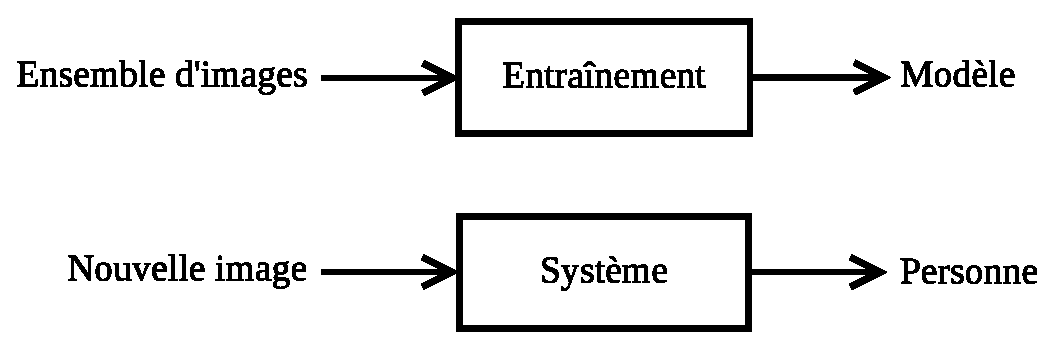
\includegraphics[scale=0.5]{images/article_etapes}
    \caption{Étapes de la méthode de \cite{article}.}
    \label{fig:article:etapes}
\end{figure}
Toutes les images sont préalablement converties en niveaux de gris.

\subsubsection{Apprentissage du modèle}
On utilise un classifieur bayésien dans lequel on suppose que $P(X_i|Y=y)$ suit une distribution
gaussienne ($X_i|Y=y \sim N(\mu_{iy}, \sigma_{iy})$).
L'étape d'apprentissage permet d'estimer les paramètres du modèle ($\mu_{iy} et
\sigma_{iy}$ pour chaque i et chaque y).
La figure \ref{fig:article:etapes_apprentissage} montre les différentes étapes
de l'apprentissage, celles-ci sont :
\begin{enumerate}
    \item À partir des images d’entraînement, calculer les eigenfaces
    comme indiqué dans la sous-section \ref{subsection:presentation_eigenfaces}.
    Ces eigenfaces forment une base de l'espace vectoriel des visages (facespace).
    \item Pour chaque image $I$ de l'ensemble d'entraînement :
    \begin{enumerate}
        \item Transformer $I$, qui est une image en deux dimensions, en un
        vecteur $\Gamma$ à une dimension.
        \item Trouver les coordonnées de $\Gamma$ dans la base eigenfaces
        (en faisant un produit scalaire avec chaque eigenface).
        On obtient les coordonnées $(x_1, x_2, ..., x_M)$ où $M$
        est le nombre d'images dans la base eigenface, qui est également le nombre d'images
        dans la base de données d'entraînement.
        \item Faire passer $(x_1, x_2, ..., x_M)$ à l'entrée du classifieur
        bayésien pour qu'il apprenne les paramètres.
    \end{enumerate}
\end{enumerate}
\begin{figure}[H]
    \centering
    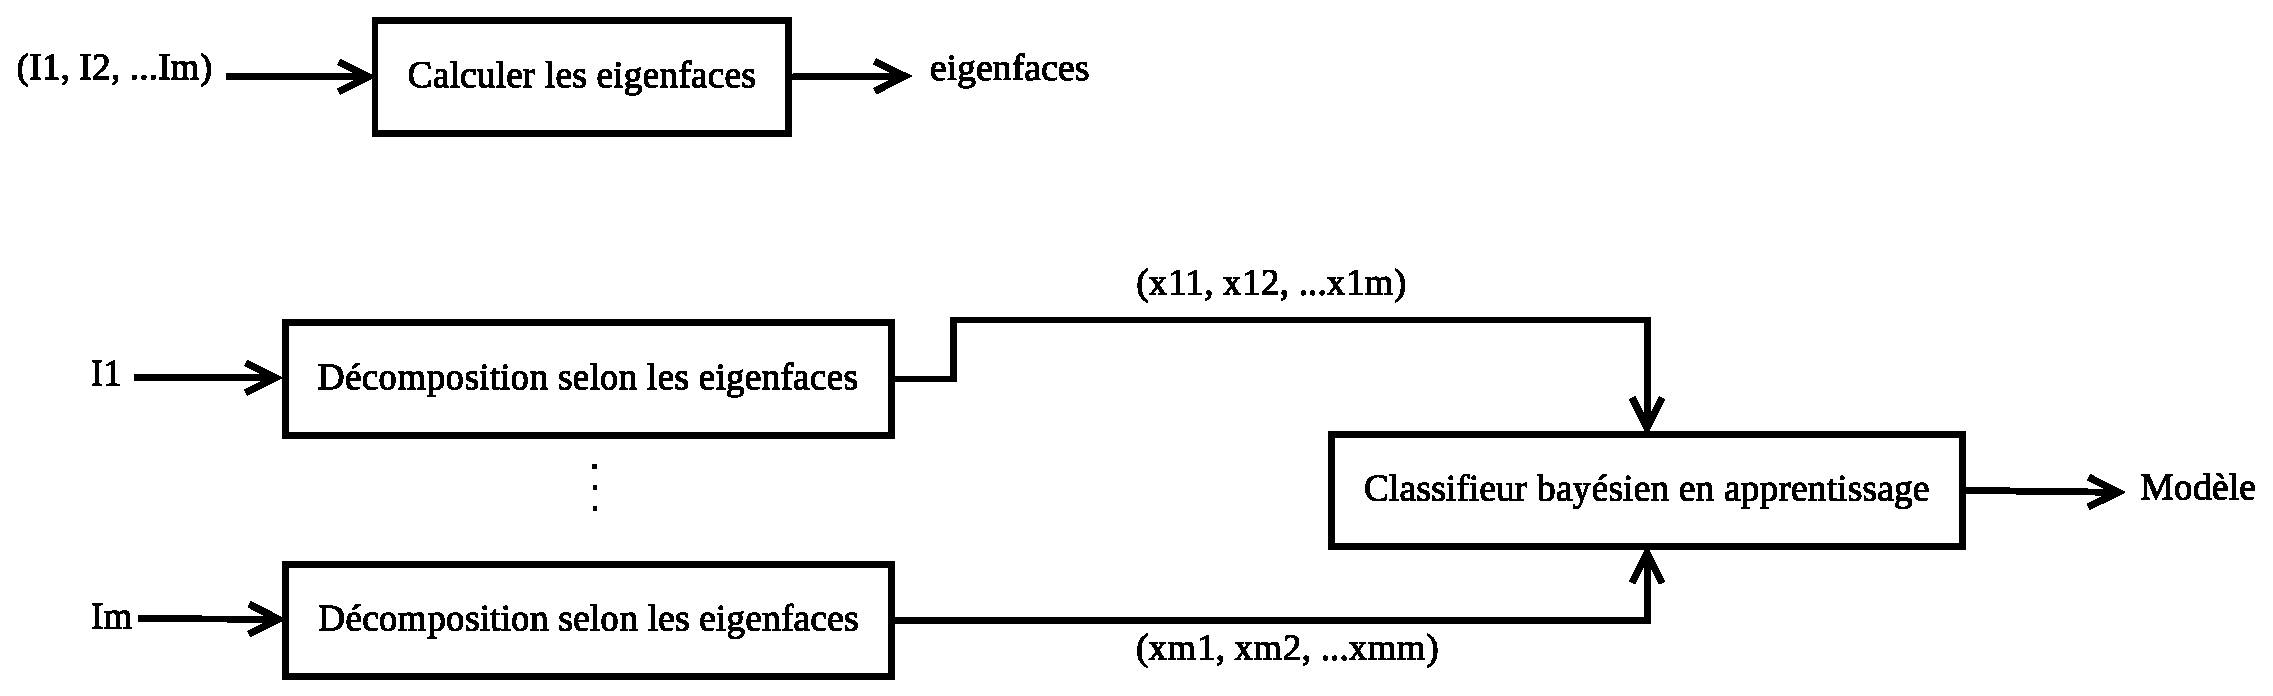
\includegraphics[scale=0.4]{images/article_etapes_apprentissage}
    \caption{Étape d'apprentissage.}
    \label{fig:article:etapes_apprentissage}
\end{figure}
À la fin de cette étape, on aura l'ensemble des eigenfaces et un classifieur 
bayésien entraîné.

\subsubsection{Déploiement du modèle}
Une fois le modèle appris, on peut reconnaître de nouvelles images. Quand on a une nouvelle
image d'un visage, on calcule ses coordonnées dans la base des eigenfaces et on fait
passer ces coordonnées à l'entrée du classifieur bayésien qui nous donne en sortie la
personne à laquelle appartient le visage. Le visage doit appartenir à une personne qui existe
dans la base de données d'entraînement. La figure \ref{fig:article:etapes_deploiement}
résume cette étape.
\begin{figure}[H]
    \centering
    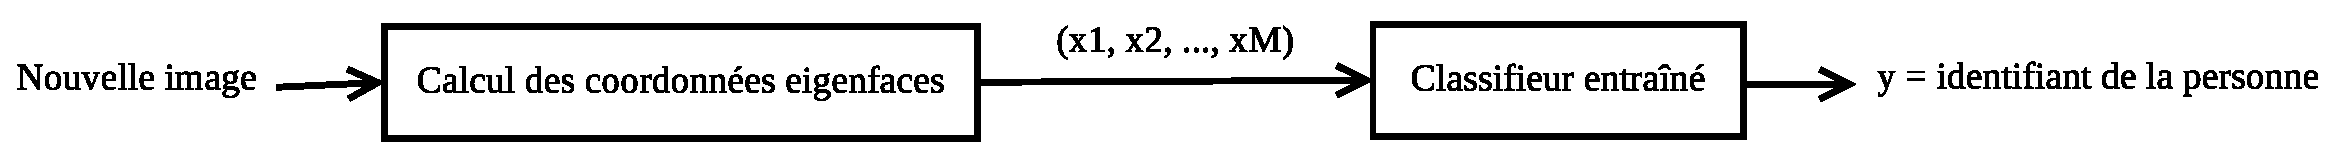
\includegraphics[scale=0.4]{images/article_etapes_deploiement}
    \caption{Système déployé.}
    \label{fig:article:etapes_deploiement}
\end{figure}


\subsection{Résultats obtenus par la méthode}
Les auteurs de \cite{article} ont travaillé sur une base de données
de 200 images de 20 personnes, avec donc 10 images par personne.
Le taux d'images correctement classées est de $70\%$. En normalisant
(centrer, réduire) les valeurs des vecteurs propres (eigenfaces),
les auteurs affirment avoir obtenu un taux de réussite de $89.5\%$.


\subsection{Critique de la méthodologie de test}
Pour le calcul des eigenfaces, les auteurs de \cite{article} ont
utilisé toutes les images de la base de données (pas de séparation
en données d'entraînement et de test). Ensuite, ils ont fait de la
validation croisée pour entraîner le classifieur bayésien et estimer
le taux de succès de la méthode. Mais étant donné que même les 
données de test ont été utilisées pour la génération des eigenfaces,
les résultats obtenus sont biaisés, les données de tests ne doivent
pas du tout rentrer dans le processus de génération du modèle.